% \textcite{} \parencite{} - are the tags for citation in apa-biblatex
\documentclass[12pt]{article}
\usepackage{fullpage} %for a school paper I am required to use only 1'' margins
\usepackage[utf8]{inputenc} %encodes fonts for Russian
\usepackage[T2A, T1]{fontenc} %also encodes for Russian
\usepackage[russian,american]{babel} %specifies the language
\usepackage{csquotes} %used with babel to include block quotes
\usepackage{quoting} %also for block quotes
\usepackage[style=apa]{biblatex} %citation system
\DeclareLanguageMapping{american}{american-apa} %note that language must match here with babel
\addbibresource{Synthesis.bib} %path of the bibliography file
\hyphenation{pho-ne-ti-cal-ly} %this avoids funny hyphenations
\raggedbottom %doesn't distribute text evenly across the page
\usepackage{footnote} %allows footnotes
\usepackage{chronology}%builds a continuum
\usepackage{array} %something cool with tables
\usepackage{titling} %better title pages
\usepackage{setspace} %has to do with spacing para's
\usepackage{graphicx} %in case i have images
\usepackage{pdflscape} %in case i need a landscape page
\usepackage{indentfirst} %indents the first row of para
\usepackage{hyperref} %references to self throughout the doc
\usepackage{multirow} %need for tables where a row may split into multiples
\setlength\extrarowheight{5pt} %extra space between rows
\pretitle{\begin{center}\Large Synthesis paper \par \vspace{30pt}}

\title{\textit{Between ethnography and conversation analysis: \\ Connecting conversational genre and person reference}}

\author{\vspace{50pt} Irina Wagner}

\postauthor{\end{tabular}\vspace{150pt} \par Committee: \\ Dr. Andrew Cowell (chair), \\ Dr. Barbara Fox, \\ Dr. Kira Hall \end{center}}
 
\date{\today}
\begin{document}
\begin{titlingpage}
\setlength{\droptitle}{100pt}
\maketitle
\end{titlingpage}
\doublespacing
\indent

\section{Introduction}
Starting with an innovative research by \textcite{moerman1988}, there have been several attempts at combining the methods of Conversation Analysis (CA) and ethnography \parencite{sidnell2008, dingemanse2014}. The main premise of such combination lays in enriching methods of CA with the background cultural and social knowledge of the speech community being observed. Since most of the early CA studies were done in English, CA researchers could rely on their own linguistic and cultural intuition in providing the most accurate description of an interaction process. With the growing interest in studying interaction in languages other than English, CA analysts have become more aware of the cultural competencies that inform conversation just as much as linguistic competencies do. However, while this divide between ethnography and conversation analysis has been bridged primarily by providing the cultural, historical, political, and social context for interaction, few analysts succeeded in using analytical tools of ethnography of speaking in their research. Meanwhile, to reach the level of collaboration between CA and ethnography of speaking, or even sociocultural linguistics, this theoretical framework must not only share the knowledge or methodology, but also develop its own set of analytical tools.

In this paper, I am bringing together a concept of genre and a  feature of person reference to bridge the theoretical and methodological gap between the CA and ethnographic research. I argue that using the sociolinguistic approaches of ethnography of speaking \parencite{hymes1974}, and the concept of ``speech genre'' \parencite{bakhtin1986}, it is possible to analyze different types of interaction as social practice depending on its structural organization and effects achieved. At the same time, the variation in person reference forms in conversations reflects the organization of the discourse as well as the cultural premises both of which become available by studying conversation more closely. Combining these two concepts into one theoretical model, I suggest that categorization of a conversation or its parts into genres can benefit the analysis of naturally occurring conversations (especially for the underdocumented languages) by guiding the analyst to understand the function of a given interaction. Person reference, at its turn, can serve as a marker of this genre. The ultimate goal of this paper is to argue that conversational genres, while being a useful analytical tool in studying face-to-face interactions, are universal categories, and that speech communities have varying speech genres which could be determined by the use of person reference forms.

The scope of the synthesis paper does not account for the original data analysis, so instead, all of the examples provided further are from relevant researches on communicative practice. Being most interested in the Native North American languages and cultures, I am using the data from a few ethnographies on the unrelated nations -- Western Apache \parencite{basso1996, basso1990, samuels2004} and Severn Ojibwe \parencite{valentine1995}. However, because there has been very little CA-type research in Native American communities, the examples for person reference come from a variety of sources, including those done in English. 

The paper has two main sections that focus on the concept and feature at question. At first, I  outline the theoretical background of genre studies and introduce the Bakhtinian concept of \textit{speech genre}. Also in this section, I  clarify the distinction between \textit{genre, discourse mode, register} and \textit{style}. The second part of the paper is devoted to person reference, which has traditionally been studied in CA as having structural and cultural premises, both of which are thoroughly defined. In the final section of the paper, I attempt to bring the two theoretical models to a dialog and propose the concept of \textit{conversational genres}. Here I provide some examples from the mentioned ethnographies. In the end, I bring conversation genres and person reference together to argue that their relationship is evident from the structure and function of a conversation.
\section{Theoretical approaches to genre}
Theories of genre dominate in the literary studies but have also been adopted in a range of social sciences and in humanities. Categorization of text or performance, approaches its analysis from two different perspectives simultaneously. On the one hand, genres imply internal structural similarities and differences. So, verse in poetry characterizes the poetic organization of the text. On the other hand, genre is also a functional categorization: a particular genre is often associated with the content and context of its text as well as the expected effect on the audience. Nonetheless, this concept is not particularly favored in linguistics due to its close conceptual proximity with other terms identifying linguistic variation, such as register, style, etc. Drawing from different approaches on genre in ethnography of speaking, linguistic anthropology, and discourse analysis, this section offers to accentuate the connection between genre and social practice.
\subsection{Speech genre}
The concept of speech genre is not a new one, and was previously introduced by \textcite{bakhtin1986} as speech genre\footnote{In the original, Mikhail Bakhtin named these \foreignlanguage{russian}{\textit{речевые жанры}} which was translated as `speech genres.' It is important to note that `speech' or \foreignlanguage{russian}{\textit{речь}} in this context does not refer to a  practice of giving speeches. Rather, this notion treats speech as a process of speaking whether it is \textit{to} or \textit{with} someone. So, in my interpretation of Bakhtin, I use the term `conversational genres' to account for the spoken aspect of speech and its interactional and emergent features.} to account for variation in style and organization of everyday interactions. When introducing speech genres, \textcite[p. 65]{bakhtin1986} compared them to ``drive belts from the history of the society to the history of language,'' with which he emphasized the historical nature of the establishment of speech genres. In order for an utterance to become typical of a speech genre, it needs multiple repetitions, polishing, and experimenting. Importantly, according to this historical approach, speech genres are intricately connected with the society who creates and judges the acceptance of a new speech genre. This discussion proposes a concept of conversational genre as a sub-type of speech genre and as an important analytical tool for the discussion of face-to-face interactions. The main goal of this concept is to interrogate them as necessary for deriving the social meaning of the full interaction. Because the conversational genres express the cultural rationale for structuring the talk and engaging in the sociocultural commentary of ideology and practice, it is argued that they are defined by culture and society itself and mimic the goals of the speech community. 

In his original framework, \textcite{bakhtin1986} distinguished primary and secondary speech genres as having a functional distinction between them. The primary ones are what Bakhtin called `simple' speech genres. Although he did not clearly define them, it appears from his juxtaposition that the primary speech genres are in fact the type of utterances that arise from verbal interactions that are not mediated and not contextualized in a particular style. Secondary, or complex, speech genres, Bakhtin argued, have roots in more organized and developed\footnote{However, I would argue with Bakhtin that any form of communication is highly organized, even though it may appear simple, e.g. conversation.} forms of communication which also often have features of artistic, sociopolitical, and sophisticated nature. Such known genres as novels, scientific research, presidential address, etc. are considered secondary speech genres as they embody a complex of ``mediated speech'' and correspond with the historical and sociopolitical contexts of their construction. With this, I can now clarify that the \textit{conversational genres} that are being investigated in this paper are the primary speech genres in Bakhtin's framework, and they correspond with unmediated oral spontaneous discourse.

In a recent study of contemporary speech genres in Russian, \textcite{dementyev2015} suggested to analyze them with regards to diachronic and synchronic features. An ability to distinguish diachronic features of a genre would indicate sequential nature of its appearance. So for example, many of the contemporary speech genres found on the Internet today are secondary to the oral communication. So an instant messaging conversation online would be considered a secondary speech genre developed from face-to-face interaction and mediated by the means of technology. Synchronic features exist in the same timeline as the discourse and are expressed in such linguistic features as register and style. The development of new speech genres is not only historically determined (especially with the secondary ones), but it also relies on linguistic processes of borrowing, semantic shift, and axiological factors. So \textcite[p. 81-82]{dementyev2015} argued that just like words or grammatical constructions, speech genres can be borrowed across languages, that their meanings can change change due to the dissonance between the factual and implied social meaning, that the knowledge of proper use of a speech genre is much more important than the knowledge of the genre itself. All of these factors that determine development of speech genres highlight that a speech genre is a complex of structural and functional elements, combination of which creates a discourse with particular social meaning grounded in the sociopolitical history of the speech community. 

\begin{table}[ht]
\centering
\caption{Parameters of speech genre according to Dementyev (2015, p. 84).}
\label{sg-parameters}
\begin{tabular}{|l p{4.5in}|}
\hline
\textbf{Parameter} & \textbf{Description}\\
\hline
\textit{Subject of speech} & indicates the main theme of a speech genre according to Bakhtin (\citeyear{bakhtin1986})\\ \hline
\textit{Style} & refers to the mode of communication which can relate either to the expressivity or pragmatics of the discourse\\ \hline
\textit{Lexicon} & is composed of the key phrases used in the genre, its unofficial name and etymology\\ \hline
\textit{Syntactic structure}& defines the composition of the discourse\\ \hline
\textit{Goal setting} & refers the projected social meaning of the utterance or discourse\\ \hline
\textit{Primacy} & whether the discourse is of primary or secondary speech genre\\ \hline
\textit{Social factor }& the value (moral or aesthetic) that the utterance or discourse have in a given community\\ \hline
\textit{General cultural paradigm} & cultural context which consists of language ideology, language policy, cultural isolation, and globalization\\ \hline
\textit{Communicational spheres} & are the modalities salient for this discourse, including the information about the participants of this talk\\ \hline
\textit{Sources of material} & historical and diachronic features of discourse\\ 
\hline
\end{tabular}
\end{table}

Outlining the methodology for studying speech genres, \textcite{dementyev2015} suggested to use a set of parameters based both on the linguistic and discursive content of speech (Table \ref{sg-parameters}). This methodology clearly bridges the gap between the functional and structural features of genre, and conceptualizes discourse as consisting of common structures, themes, modalities, styles, while pursuing a particular social goal in the ever-changing cultural context. As an example, \textcite{dementyev2015} analyzed a speech genre of `heart-to-heart conversation' (\foreignlanguage{russian}{\textit{разговор по душам}} which is a common conversational speech genre practiced as a form of intimate talk between any acquainted or not acquainted people. In his analysis, Dementyev limited his data to the instances of it appearing online on discussion forums and found that nearly all parameters of this speech genre are mimicked online. There are three features that he emphasized as crucial for this speech genre: the axiological nature of this talk, lexical component, and the participants of talk. So from the point of view of the value of such type of talk, he found that heart-to-heart conversations are crucial to people sharing this cultural value. In particular, grounding this practice in the traditions of Russian culture, he analyzed this speech genre as pervasively positive based on his data. Only some negative connotations of it surface when such speech genre is juxtaposed in the social contexts of modernity. Structurally speaking, the researcher argued that such conversation almost universally begins with one of the speakers saying the key phrase (and some of its variations) \foreignlanguage{russian}{\textit{Что же на душе так хреново / погано / паршиво?}} `Why is my heart so heavy?' (p. 100). In face-to-face conversations, Dementyev postulated, such  opening acts as  invitations to an intimate conversation. Online, he found, it has a similar goal: it invites other forum users to initiate a conversation, ask what happened, sympathize with the person who is feeling down, and cheer them up. Unlike in face-to-face conversations, the medium of the internet which allows asynchronous and anonymous communication also licenses rude responses that would be at least frowned upon (if not impossible) in face-to-face talk, e.g., a symmetrical complaint (\foreignlanguage{russian}{\textit{а у меня не лучше!} `my life isn't better!'}) or an advice (\foreignlanguage{russian}{\textit{забей!}} `forget it!'). In other words, by changing the communicative sphere of this speech genre and extending it on the web, speakers fulfill the requirement of talking to strangers, but also encounter hostility and dispreferred responses. In general, the purpose of such genre is phatic communication, and it is achieved regardless of the medium.

Other important components that Dementyev distinguished in his research are the \textit{dominant} and the \textit{norm} of a genre. \textit{Dominant} can be loosely defined as the semantic or pragmatic head of the communication, its driving feature. So \textit{heart-to-heart conversation} has a dominant of \textit{sincerety} (when speakers engage in this practice, they hope that the conversation remains serious and sincere which contribute to highly moral evaluations of this type of talk in the Russian culture), whereas \textit{small talk} has a dominant of \textit{politeness} (p. 85). \textit{Norm}, on the other hand, seems to define the patterns of talk and its sociocultural context. So, norms of \textit{heart-to-heart talk} would include \textit{conditional routine, familiarity, trust, and simplicity}, whereas \textit{small talk} is defined by \textit{formality, friendliness, and strangeness}. Dominants and norms can be useful features in understanding the goal of speaking as their corresponding matching between the expectation and reality would indicate the overall tone of the conversation. These parameters in general can bridge the divide between the speech genres and speech acts -- the intentions of an utterance. 

In sum, speech genres can be defined as spoken utterances exhibiting consistent structure, repeated in same social, historical, and cultural contexts and thus yielding a particular social meaning. Defined by a set of parameters, speech genre are also common expressions of cultural expectations of interaction, which can be traced in the form of a dominant and a norm. Having outlined the working definition of speech genre, I will now discuss its relation to other components of spoken discourse.
\subsection{Genre vs. register}
In linguistics, the focus on the metaprgmatic and metalinguistic aspects of text conflates genre with speech events and register, which prompted \textcite{swales1990} to report that linguistics generally finds genre ``indigestible'' (p. 41). \textcite{hymes1974} also noted this conceptual similarity but argued that genres and speech events are different analytical tools: while he restricted speech events to the activities governed by rules for the use of speech, the concept of genre he associated with types of speech sharing similar structures but being invoked at various situations. In his understanding, genre lacks functional component and texts and performances of same genre can be used with the same effect in different situations. As \textcite{swales1990} noticed, this approach would mean that when a sermon is given outside of a funeral for satiric or political purposes, it remains to be a sermon with all of its effects and meanings. Meanwhile, according to \textcite{bakhtin1986}, thinking that a genre remains same in different contexts, disregards the conventionalism and intertextuality as the essential features of genre and even lack functional properties. By emphasizing the functions and conditions of speech and utterance, \textcite{bakhtin1986} suggested that genres appear in response to speech, differentiating self from style and grammar.  

Similarly, the functional distinction seems to be a major aspect of confusing register and genre. \textcite[p. 191]{biber2012} defined register as ``text varieties of a language associated with a particular situation of use,'' also suggesting that register corresponds with the differences in linguistic features according to the desired function of text. In order to differentiate it from genre, Biber suggested that genre analysis looks ``beyond the sentence'' unlike the studies in the register. Furthermore, he proposed also to distinguish the functional and conventional functions of genre: since both register and genre are defined as language variations dependent on the accomplishment of a particular effect, the main difference between them is that of a conventional use of genre. In other words, Biber argued that linguistic variation according to genre is socially expected to conform to particular rules of language use rather than distinct situational contexts. 

Following the ``Hallidayean'' approach to genre, \textcite{swales1990} further disambiguated this distinction, stating that register and genre are on different levels of analysis. Register is described as \textit{a tripartite system} in which each part (field, tenor, mode) responds to different level of text management (correspondingly: ideas, personal relations, and discourse). Importantly, the realization of the text management on each level can only be accomplished by language. Consequently, genre is proposed to be ``underlying to register'' -- a level on which things get done \parencite[p. 40]{swales1990}. Thus, the relationship between genre and register is complementary, each of them is chosen independently in order to achieve the predetermined social goals.

Thinking of genre, \textcite{bakhtin1986} argued that generic differences appear from repetition of speech or utterance in different contexts. This view also suggests that it is nearly impossible to find such a speech or utterance that has not yet been produced to some degree at some time. Yet, what makes it different each time is the manipulation of the content by speakers to ensure expected outcome of the speaking. So, narrative genres in particular, \textcite[p. 181]{hyvarinen2015} suggested, ``function as frames of orientation for the language users themselves within certain social practices.'' In other words, the main advantage of employing genre in analysis is the ability not only to categorize text or performance, but also to observe their meaning and reception by a speech community. Ultimately, use of a particular genre in speech leads to creating and maintaining social practice by its employment of intertextuality \parencite{briggs1992} and iterdiscursivity \parencite{wortham2015}. \textit{Intertextuality} can be defined as a structural principle of textuality that remains constant or recognizable across speech events \parencite{wortham2015}. Being produced and reproduced, distinguishing attributes of text may have specific effects in the speech community by triggering the available ideologies and relating them to the previous discourse \parencite{bakhtin1986}. \textit{Interdiscursivity} specifies how ways of talking can establish chains of speech events, and eventually become associated with certain social types and evaluations creating the trajectories of accomplishing social processes \parencite{agha2003}. Having the intertextual knowledge, audience is able to produce the appropriate reaction to text or a performance, which can be either realized in action, a verbal response, or even rejected. So, manipulations of genre are available not only to the authors, who can mix different ones and change the expectations of a reaction for the effects of humor, for example, but also to the audience who may not recognize features of intertextuality and reject the text \parencite{bax2011}. Importantly, the expectation of a reaction indicates the field of possibilities based on the previous talk. In other words, every speech or utterance in the Bakhtinian view is ``linked'' to other ones that have come before it either verbally or orally \parencite[p. 69]{bakhtin1986}

\subsection{Genre vs. discourse modes}
A step toward creating a list of genre lays in the understanding of the varieties, conventions, and purposes of communication. So, the idea of discourse modes as the possible varieties of these processes describes distinct possibilities of using written and oral text for the purposes of achieving different contextual effects. \textcite[p. 54]{bax2011} explained that discourse modes are different from genre in a more abstract, pre-existing sense, by defining the possibilities of using the language rather than simply extracting its semantic meaning. Depending on the approach to discourse modes, they are usually recognized by what they are attempting to do: narrate, describe, and argue. An additional mode that is often included in this list is conversation, or dialog, which is also often conceived to be the essential abstract form of human communication \parencite{bakhtin1986, bax2011}. Considering the research on discourse modes, discourse modes, genres, and register are related to each other in a nested hierarchy, in which each dominating level makes use of the properties and features of the category below. In this hierarchy, genre consists of discourse modes which roughly could be thought of as suprasegmental features of register.

Because narrative and interaction are considered essential in communication, they are highly accessible and available to all interlocutors.  In fact, when trying to outline discourse modes, \textcite{georgakopoulou2000} simply distinguished between narrative and non-narrative discourse. The simplicity of such an approach may not account for the variation in arguments and interaction, yet, it emphasizes the primacy of narrative in the everyday communication. Narratives fulfill multiple functions in our social activities, including socialization, processing of events, organization of the community, and ensuring the cohesion of the culture \parencite{georgakopoulou2000}. The term ``narrative'' is being used in its broadest sense as a rhetorical mode that recounts or represents ``some temporally instantaneous event'' (p. 123). The main defining feature of this discourse mode is its referentiality: informed by the context of an interaction, narrative attempts to reconstruct the reality while non-narrative, or conversation, aims to verify or validate it. So, one thing that non-narrative modes, such as conversations, have in common is their tendency to establish truth by the means of different interactional techniques, such as interrogation, evaluation, argument, etc. While these techniques are also available in a narrative, they cannot be used without reproducing a durative event in the heights of the story. 

%re-write
Textually, both of the discourse modes differ in the pattern of their structures. \textcite{bakhtin1986} proclaimed dialog the most basic form of communication due to the simplicity of its structure: turn-taking in conversation, according to them, creates clear-cut boundaries between utterances while also maintaining the contextual relationship between them. So, speakers are aware that after a question in a conversation, the answer follows which demonstrates rigid organization not observed anywhere else in language\footnote{That is, a speaker cannot with full certainty predict what will follow after a word or a sound has been produced. The foreseeable relationships have only been described with regards to some colloquial terms and indioms and face-to-face interaction.}. However, in  narrative, a different structure emerges, indicating a specific pattern characteristic to this discourse mode. Because of its attempt to reproduce durative events in somewhat time-related manner, narrative discourse tends to have an internal time sequence organization that can be narrowed to orientation, complication and resolution \parencite{labov1967}. Additionally, non-narrative discourse uses a variety of features to organize itself, such as intonation, gaze, gesture, anaphora, pauses, interaction-specific syntax, etc., while narratives rely primarily on the features of its content (time, place, characters), rhythmic units, such as verse and stanza, and inferred or explicit causal connectors (Georgakopoulou and Goutsos 2000). With these considerations in mind, one would also expect more fine-grained distinctions in the way each of these modes uses language: in particular, with regards to style and register. 

Having outlined the main concepts of each of these two discourse modes, I must also note that these modes are not exclusive, since conversational narrative is also a possibility that comes with a variety of its own structural, contextual and referential features. \textcite{norrick2000} indicated that sequentiality of time, while often relevant, can be omitted in the narrative to appeal to a particular point. Moreover, the boundaries of a narrative are much less distinctive in a conversation because the narrative pattern may not follow the expected route (e.g., in a collaborative conversational narrative the sequence of events can unfold in a non-linear order) and may not have distinctive boundaries even in the beginning and the end. Yet, previous research on conversational narrative showed it to be a particular type of discourse differentiated from other modes with register unraveling some of the minor differences between them.

In general, when talking about discourse, the previous research argued that it consists of different levels of performance differentiated by the function and structure of talk together contributing to the creation of social meaning. Discourse modes, unlike genre, outline only the contextual and textual features of the text which normally refer to the general structure and specific devices that it uses. Unlike genre, discourse modes are not patterned by agreed-upon conventions and do not influence social practice. On the opposite, they merely function as a frame of text presentation. Registers, on the other hand, function as minimalistic representations of linguistic variation. By employing certain linguistic repertoires and varieties depending on the context, registers add metalinguistic information to the text. Genres are said to be in the intermediate level of text production as they combine the information provided by the registers and apply it within a particular discourse mode. Speakers know how to alternate structural composition of text in order to achieve a particular response from the audience. Conceptualizing genres as conventional mental schemes, this approach accentuates the role of society in the production and reproduction of genre. In a sense, genres are presented here as ``socially endorsed'' \parencite[p. 60]{bax2011} as though only the speech community can agree upon their functions and features, while individual speakers have no control over them.  
\subsection{Genre as social practice}
The intertextual nature of genre proves a strong connection between discourse and practice. In connecting genre to social practice, \textcite{hanks1987} insisted that genres actually form the \textit{linguistic habitus} of a speech community. In particular, he noted that genres cannot persist without the community who understands its conventions, intertextuality, and social meaning, which allows them to be recognized as the core of social practice. As an action within a community of practice, genre is conditioned by a set of symbolic characteristics forming a mental schema shared by the representatives of the community. Thus, Hanks concluded, genres like any other schema exist prior to any event of practice, organizing the linguistic habitus and yet prone to change and innovation with the changes in the society.

The variations in text and commonality in genre categories indicate that the two of them are different concepts of presentation. Text, being determined by registers and styles of speech, is a concrete product, whereas genre is only ideational because it can only outline or frame the main concepts of text depending on the context and the audience \parencite{bax2011}. The convenience of genre is expressed by its classificatory functions of text and in its overwhelming applicability to different types of speech events. Genre ultimately allows to distinguish similar patterns in structure, expectations, and presentation of text, and categorize texts with similar features together. The complexity of text, however, shows that genre categorization is not as unequivocal as it appears to be because of the fuzzy boundaries of textual categories and the possibilities of genre mixing. The capability of authors and speakers to mold their text in response to a varieties of factors makes hybridity of genres inevitable and complicates proper categorization of texts \parencite{bax2011}. On the other hand, \textcite{bakhtin1986} saw genre hybridity, or as they called it ``flexibility,'' as an inherent feature of communication. The creativity of speakers is essential in communication, which leads to pure impossibility of a comprehensive list of all of the speech genre. At the same time, they noted, that the better knowledge of genre opens up better possibilities in more ways of using them for social communication.

%perhaps talk about the political text and such of Duranti? Greetings vs other oratory expressions?

So, while defining ``genre,'' some of its features must be especially emphasized in order to distinguish it from other linguistic concepts such as speech event, register, style, and mode. What comes from the discussion above is that key aspects of genre are its functionality and conventionalism. So genres, unlike other concepts, perform particular discursive functions and are defined by socially accepted conventions on the presentation of the text and the proper reaction to it. Because of this strong connection between genres, conventions, and speech community, genres are argued to form part of the linguistic habitus of a speech community. Genres are also defined by their particular structures, which conform to the previously known productions of text. In their construction, genres can use a variety of linguistic devices in order to correspond with the appropriate expectations for production and reception, such as particular registers, styles of speaking, and varying grammatical features. At the same time, correlations of registers and genres can also indicate the successful comprehension and effect of text on  social practice. With that, it is important to highlight that the connection between genre, registers, and styles of speaking is often mutually reinforcing and complex. 
\section{Approaches to person reference in conversations}
The feature of person reference is a well-researched topic in conversation analysis. Besides being interesting from the point of view of membership categorization, person reference is also a useful indicator of internal structure, recognitionality, and semantic frameworks available in the conversations. Although most of the research in person reference have been performed on English and English-speaking communities, some recent studies also looked at referring practices in lesser studied languages and their communities of practice, expanding our view on the principles of referentiality. In general, there seems to be an agreement between the researchers that person reference has both structural and cultural principles behind their choice. Here, I would like to discuss the logic for the principles in the current research. I aim to demonstrate that beyond their grammatical, structural, categorizing, and referential principles, terms of person reference also play key role in identification and construction of the conversational genres.

In selecting a form of person reference, speakers rely on the conversational structure as well as familiarity of the interlocutors with the referent. The research on this subject demonstrates several significant attempts to describe the principles of that choice which can be roughly narrowed down to structural, cultural, and grammatical principles. Importantly, previous studies tend to use these principles as competing self-sufficient theories, rather than a highly structured model defining the selection in a conversation. In the following discussion of the existing theories, I will argue that person reference is a complex feature of a conversation which manifests the cultural grounds of any interaction.
\subsection{Structural premises}
The two major principles underlying the choice of person reference terms are described in their landmark study by \textcite{sacks1979}. According to them, a successful term of person reference should be short but at the same time semantically full to be recognized from the first attempt at pronouncing it:
\begin{enumerate}
\item ``On occasions when reference is to be done, it should be preferredly be done with a single reference form.''
\item ``If they are possible, prefer recognitionals.'' (p. 24)
\end{enumerate}
Having enumerated these principles, Sacks and Schegloff, nonetheless, emphasize that recognitionality is most important and must be achieved first. They argue that ignoring the principle of recognition may cause extra work of disambiguation to the speakers and become counterproductive in conversations. In general, recognitionality or recognizability implies that in any given moment in conversation the speaker must be aware of the knowledge of the referent by the addressee. This statement makes recognitionality a feature of recipient design that can structure conversation by implications of shared knowledge or by requiring additional clarifications and disambiguations. 

The term ``recognitional'' is a vague one and can be better described by the speaker's presupposition of addressee's knowledge of the referred person. While it is often equated to ``identifiable,'' the two have different properties. ``Identifiable'' is a term applicable to objects and subjects that are uniquely distinguished from one another \parencite{clark1986, chafe1976}. ``Recognitional,'' however, refers not just to the identification of the object, but also connotes the shared mutual knowledge of the object's properties \parencite{clark1986, defornel1987, sacks1979}. As \textcite{chafe1976} notes, for something to be recognitional, it needs to be semantically available in the domain of talk. So, for a speaker to use a reference to a person not previously brought up in the conversation, there needs to be substantial semantic and pragmatic background already shared with the addressee. An example often cited from \textcite{schegloff2007} is the anaphoric use of the third person singular pronoun when speaking about John F. Kennedy shortly after his attempted assassination. While ``he'' is an identifiable pronoun, the reference is recognizable because shortly after the event, the tragedy was on the minds of many people in the U.S. and ``he'' was a mutually shared understanding of the President. In sum, recognitionality of a referent is a collaborative achievement: while the speaker must make such a referent identifiable based on the understanding of shared common knowledge, the addressee either must provide information beforehand about the possibility of understanding, or must recognize that reference without needing additional disambiguation.

The principle of recognitionality is tied in with the structural properties of a conversation which can determine the more preferred form of reference. In her study of the anaphoric reference, \textcite{fox1987} demonstrated that a speaker would not use a minimal reference term unless that referent has already been introduced and reoccurs in the still open sequential construction. Fox argued that interlocutors track whether the sequence is still closed or open before they choose the appropriate form of person reference, demonstrating the dependence of the reference term on structural organization of the conversation. Employing the concept of ``return pop'' borrowed from natural language processing, Fox explained how the structure of a conversation can be understood and negotiated by the interlocutors. So, a minimal reference term such as a pronoun is not just the indicator of an open sequence, but it can also mark the importance of the closed adjacency pair for the conversation by reintroducing the same referent anaphorically. In a sense, the organization of non-story talk is activated by the person reference terms and is also shaped by them.   

Similarly, in a different research \textcite{schegloff1996b} also demonstrated the connection between the forms of person reference and the structure of talk. In order to define preferentiality in the form of reference, he distinguished between initial and subsequent terms and positions. According to Schegloff, the main structural difference between the reference forms is their appearance in talk. So, he identified \textit{locally initial forms} as reference terms that name the referent for the first time (i.e., full noun phrases or names) and\textit{ locally subsequent forms} as the terms of reference that merely point back at the already identified and recognizable referent (i.e., anaphoric devices such as pronouns). As he demonstrated, the coordination of the position of reference in talk and the term of reference has implications on the structure of the conversation. Table (\ref{form-position}) summarizes Schegloff's findings with regards to matching and mismatching the positions and reference forms.

\begin{table}[]
\centering
\caption{Structural features of reference forms and positions according to Schegloff (1996).}
\label{form-position}
\begin{tabular}{l|l|p{2in}} 
& \textbf{Locally Initial Form}                                                                                                                                         & \textbf{Locally Subsequent Form}                                                                                                                             \\
\hline
\\
\multirow{3}{1in}{\textbf{Locally Initial Position}}&  & - availability of the referent to both interlocutors;\\ & {Preferred}                                                                                                                                                              & - indicates continuation of talk;\\ & & - re-opens the sequence.\\
\hline
\multirow{4}{1in}{\textbf{Locally Subsequent Position}} & - indicates sequence boundary;\\ & - shows disagreement;\\& - often a recycled element in the overlap;& {Preferred}                                                                                                                                             \\ & - used to restart a term. 
\end{tabular}
\end{table}

Importantly, while Schegloff notes that mismatch in the position and form is possible, he argues that it is a conscious choice of a speaker who offers more than just a simple reference term. Reference \textit{simpliciter}, as \textcite[p. 1307]{hacohen2006} describe it elsewhere, is the most essential function of a reference term which does ``just referring'' and nothing else. The additional meanings of reference can include negotiation of conversational structure, disagreement, change in a speech act as well as membership categorization of a referent. In outlining the preference for locally initial and subsequent forms and positions, \textcite{schegloff1996b} is precisely referring to these potential functions of a disprefered reference.

When it comes to the potential forms of reference, the variations in the English language are plenty, and there could be even more in other languages and speech communities. In general, they can be differentiated into descriptive, neutral, and anaphoric mentions. As it follows from the discussion above, \textit{anaphoric} mentions are usually the ones that do not require establishment of an identity of the referent, and thus, they most often appear in the subsequent discourse. In English, examples of anaphoric mentions include third person pronouns (\textit{he, she, they}, demonstrative pronouns (\textit{this, that}), and some combinations (\textit{that guy}). \textit{Neutral} reference terms would be names, or somewhat arbitrary terms for referring to people that do not convey any additional meanings of empathy, for example, \textit{Bill, Mrs. Simpson, Mr. President}\footnote{However, it is also possible to argue that this categorization is rather simplistic, and even such terms of reference that appear neutral often carry with them an additional meaning, provided by the prefix of address, or a qualifying adjective. Often the difference in neutral forms of person reference (e.g., full name vs. first name) reflects politeness levels and familiarity of speakers with such referents \parencite{downing1996}}. \textit{Descriptive} terms, however, go beyond establishing the identity of a referent and introduce membership categorization, stance, affinity, physical presence, linguistic presence, etc. -- creating the ``semantic silver lining'' of person reference \parencite[p.132]{defornel1987}. The main difference between reference by name and reference by a descriptive term is that descriptors tend to attend to a property of a referent, also offering a judgment of the person and evaluating that mentioned property. Essentially, descriptive and neutral terms of reference are not interchangeable, and \textcite[p.136]{defornel1987} suggested that they operate based on the third principle of preference for the relevant role: ``choosing the relevant role is at the same time tacitly bringing into play contextually appropriate properties which are linked to the role within a social frame.'' In other words, the choice between name and descriptor relies both on successful recognitionality and the sufficient information conveyed by the term. Since names are empty of property evaluations, they cannot be used in certain speech acts.

In general, names are the preferred first time reference term in English conversations because they offer the most economic reference to a person and yet the most recognizable reference to a person \parencite{downing1996}. As Downing points out, names are a unique reference term category which can only be employed when the speaker is certain of identifiability of the referent. It means that using a name by itself can prove useless either to such interlocutors who do not know the referent by name or to such situations where referent has not yet been ``activated'' (p. 97). In such situations, speakers may use a full proper name or modify it by adding a noun phrase. In addition, speakers are shown to have other devices available to signal uncertainty about identifiability, such as try-markers \parencite{sacks1979}, noun phrases, or even explicitly negotiate the identifiability of a referent. The latter can be done by informing the addressee about such uncertainty before bringing in the proper name reference:

\begin{figure}
\caption{Explicit negotiation of referent's identifiability (Downing 1996, p. 100).}
\label{Downing}
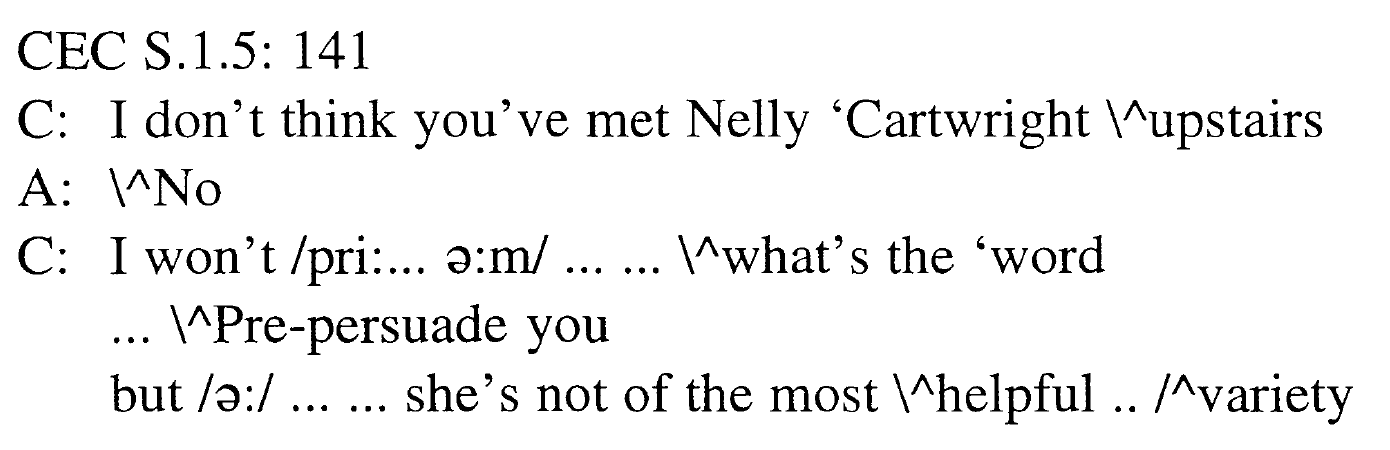
\includegraphics[width=5in]{Downing.png}
\end{figure}

The pre-introduction of the reference term in the first utterance serves to avoid identifiability issues caused by the use of a full name. In general, reference by name is an important linguistic feature as it has a meaning beyond the communicative understanding: using names not only identifies new referents in a conversation, but also outlines the knowledge boundaries of both interlocutors. In other words, personal names while serve to be the default terms of person referent, are also incredibly useful markers of epistemic stance.

As default reference forms, names serve few pragmatic functions in the conversation. In her study of ``alternative recognitionals,'' \textcite{stivers2007} demonstrates that speakers tend to use these types of reference when accomplishing a particular social action. She argued that some reference forms are a better fit for some speech types because by using such terms, speakers are able to claim a certain degree of familiarity with the referent and even align or misalign with them. So, while names are neutral and can be used across different speech acts and social situations, some references, for example, kinship terms with possessive personal pronouns become especially useful for affiliating with the referent or the speaker depending on the task being accomplished. In the following example Stivers demonstrated how such disaffiliation with the referent can be achieved by placing him in the responsibility domain of the addressee with the second person possessive pronoun:

\begin{figure}[h]
\caption{Example of disaffiliation from the referent (Stivers 2007, p. 80).}
\label{stivers}
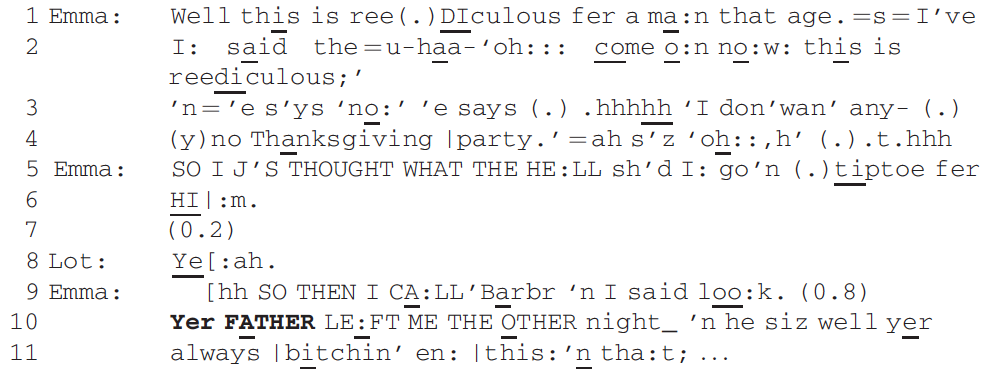
\includegraphics[width=5in]{stivers.png}
\end{figure}
While a neutral term `dad' is also possible here, Stivers argued that it would have not achieved the same result because it would have not framed the utterance as a complaint. So, the speech act of complaint is intensified by using this alternative recognitional form. In sum, this study suggests that person reference is not just a semantically loaded expression in the conversation, but it is a tool used in conveying social meaning. 

This summary of the research arguing for the structural premises in person reference demonstrates the depth with which this topic has been studied. While all the mentioned works argue for the connection between the form of reference and their relative position in the conversation, it becomes clear that speakers use reference terms beyond referring to manipulate the flow of the conversation and take certain conversational positions. The three principles that have been mentioned thus far, principle of recognition, economy, and role relevance, shape the reference term in accordance with the already available information conveyed by the organization of talk. However, as other research shows, some cultural principles also play a major role in establishing the reference even though they are usually perceived independent of the conversational structure. 
\subsection{Cultural premises}
Research on person reference in languages other than English also demonstrated that besides these structural principles, culture also affects the types of reference forms. Some of such principles recognize the difference in person reference terms that may be more amicable (such as ``mommy'' instead of ``my mother''), that may stem from bilingualism of the speakers (``John'' vs. ``Juan''), that may be defined by avoidance rules, that are differentiated in the community due to multiple names policies, etc. In general, these restrictions can be summarized by the principles of \textit{circumspection}, introduced by \textcite{levinson2007} and \textit{association}, introduced by \textcite{brown2007}. Along with the structural principles, they form a system of person reference that is argued to be common across languages yet variable across cultures. In the following pages, I will outline the main ideas behind the cultural preferences and contextualize them in the research on their relative competition in conversations.  

The existence of these two cultural principles reflect constraints on expression of relationships between people in a given community. \textit{Circumspection} is a response to the rules of avoidance in the community, and \textit{association} is a response to valorization of kinship. While they are both restricting principles, which means instead of fully identifying the referent they tend to restrict the set of possible referents, they are complementary \parencite{blythe2009}. So, unlike principles of minimization and recognition, circumspection and association do not compete, rather they aid each other in restricting the reference. With regards to their collaboration with the structural principles, the competition between all principles is determined by cultural predispositions. This means that different speech communities prioritize some principles over others in establishing reference, which can only be described in terms of salient features of person identification \parencite{enfield2013a}. 

Avoidance type relationships are said to form the principle of circumspection. This principle prescribes to ``show circumspection by not over-reducing the set of referents explicitly'' \parencite[p. 31]{levinson2007}. This principle suggests limiting the number of the possible referents due to the avoidance or taboo rules common in a specific culture. As Levinson explained, in some of the indigenous Australian cultures, there are taboos associated with the dead that would not allow one to pronounce any lexical item phonetically close to the dead person's name. Or on some occasions one would not want to fully identify the person because it may cause an adversary effect (e.g., punishment for doing something wrong or start an unwanted gossip). Instead speakers would rely on vague hints or general descriptors to establish reference. 

In general, the principle of circumspection can be understood as going against the grain from the principle of recognition outlined by \textcite{sacks1979}. \textcite{levinson2007} clarified, however, that all these principles are applied together and together they optimize the person reference. So, by aligning the types of possible references from the most ambiguous (pronouns) to the most restricted (names), Levinson suggested that each of these principles pulls the selection to different direction in order to find the most appropriate reference term: while the principle of the recognition directs the speaker to use the types of references that are most recognizable, such as kin terms or names, the principles of economy and circumspection pull this choice towards the less recognizable and more ambiguous terms.
\begin{figure}[h]
\caption{The process of competing principles in person reference (Levinson 2007, p. 34).}
\label{chart}
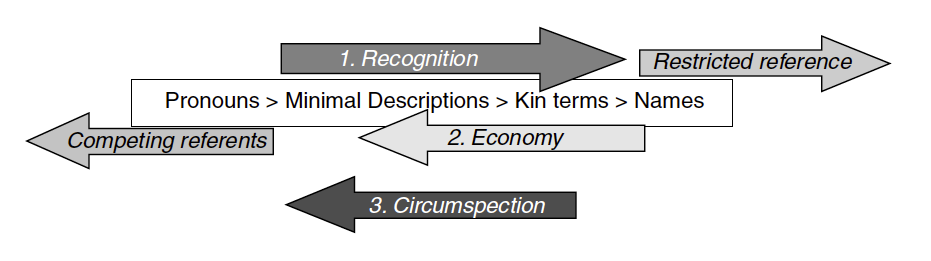
\includegraphics[width=7in]{chart.png}
\end{figure}
These principles are still not ideal in reference, and Levinson demonstrated it with his analysis of other-initiated repair. So, when a reference term is used but it is still ambiguous the addressee can ask the speaker to clarify it. According to Levinson, due to the principle of circumspection, speakers slowly upgrade a reference term turn-by-turn only if necessary:
\begin{figure}[h]
\caption{Upgrade of reference term in Yélî Dnye due to circumspection principle ambiguity (Levinson, 2007, p. 58).}
\label{levinson}
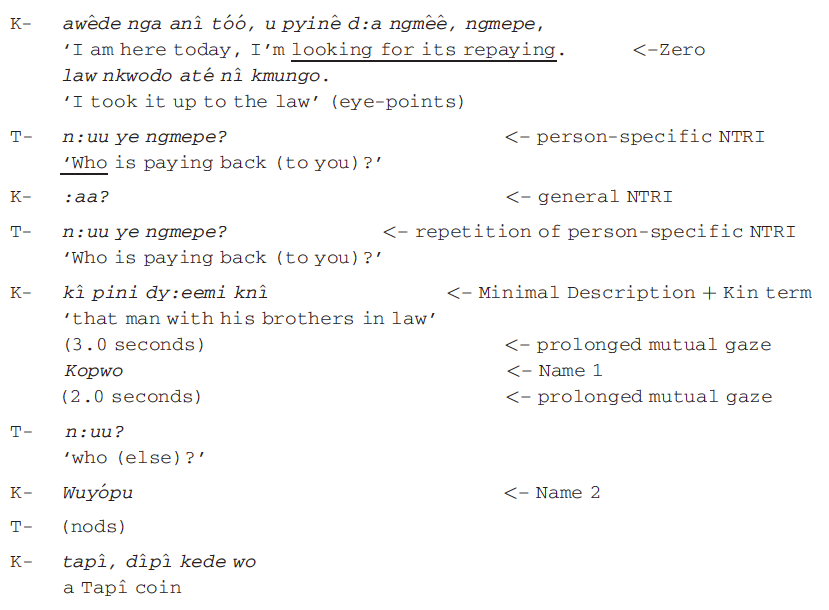
\includegraphics[width=7in]{levinson.png}
\end{figure}
The example in Figure (\ref{levinson}) demonstrates escalation of the person reference term from ``zero'' in the first utterance to a descriptive term due to the other-initiated repair (\textit{n:uu} `who') and later to a name due to subsequent misunderstanding signaled by gaze. So, while the cultural principles of avoidance are followed in avoiding the referent directly, the principle of recognition takes over causing the ambiguity and leading the speaker to clarify the reference. According to \textcite{levinson2007}, the principles forming person reference are closely interconnected and their balance is best observed in the default references such as first names in the English-speaking cultures and kin terms in some others.  

In general, the cultural principles determine the default types of person reference, and the deviation from the unmarked has been studied as conveying additional social work. In her study of non-minimal types of reference in Tzeltal, \textcite{brown2007} outlined the default reference practices and ties them with another principle – association: ``associate the referent as closely as possible to the current conversation participants'' (p. 200). Unlike in English, in Tzeltal kin terms are the unmarked or default forms of reference to people in conversations which, Brown argued, causes the formulation of the new principle. So, it is preferred to refer to a person in such a way that would establish the connection between the referent, addressee, and the speaker. If one cannot formulate such a reference term, then it should be done by displaying the kin relation of the referent and the addressee. Although such references may violate the principle of economy, Brown argued that it is more important in that social community to establish the relationship in favor of recognition. 

Studying Yucatec Maya language, \textcite{hanks2007} argued that an appropriate reference is determined by a set of cultural and discourse factors. While the descriptive terms are unmarked in this language, similar to Tzeltal, the kin terms are the default forms of person reference. Yet, the way that one would choose to establish the relationship depends on the type of relationship, associated respect, participation framework in the interaction, and the discourse context of the reference. So, to define a \textit{propositus} of the kin term, or the point of reference, the speaker essentially needs to decide which social background information is the most relevant to the talk: person reference is a ``construal of person'' \parencite[p. 149]{hanks2007} which in individuating the referent attends to the shared background knowledge of the speaker and the addressee about them. This means that by the construction of a reference term, the speaker also negotiates important matters of the subject's identity, chooses to claim a relation or responsibility to them, and defines the overall social discourse of the talk. The practices described for the Yucatec, and especially the discussion of emotions of respect evoked by kin terms of reference ground the association principle. However, in his discussion of Yucatec person reference, Hanks does not speculate on the social functions of certain names or reference terms, leaving this important issue unattended.

Working with another Mayan language community, \textcite{haviland2007} studied the possible alternatives in reference in Tzotzil. Having found that kin terminology is also the default form of person reference, he argued against \textcite{schegloff1996b} and suggested that reference is never simple, but it is always used to index social relationship -- ``referring dupliciter'' (p. 232). The data that he examined perfectly demonstrates that each mention of a person reference tends to create a projection of relationship between the speaker, the hearer, and the addressee. In fact, one of the most important findings of this research foregrounds the principle of association suggesting that it is, perhaps, the most fundamental principle in reference.

The possibility of discerning the meaning from a marked form of reference has been already discussed along with the structural principles. In a study of reference variation in Murriny Patha conversations, \textcite{blythe2009} added that reference introduces meaning both on macro and micro levels of discourse. Besides merely creating references through association, speakers also express their stance towards cultural values, such as clan membership. So by choosing a form that corresponds with the principles of circumspection and association simultaneously, speakers also define their own position towards the cultural prescriptions of avoidance while placing the referent in the recognized network of social connections.

With regards to the meanings invoked by some forms of person reference, in addition to the phenomenon of alternative recognitionals \parencite{stivers2007}, a new concept \textit{avoidance recognitionals} was introduced to account for the restrictions of references accomplished by the cultural principles \parencite{blythe2009}. Since speakers of Murriny Patha, like the speakers of the mentioned Mayan languages make up a relatively small closed community in Northern Australia, roughly any type of identifying construction can be considered recognitional. However, existence of avoidance rules leads to using avoidance recognitionals -- the type of ``recognitionals that are used when a referent's name is restricted and ``avoidance'' needs to be performed'' \textcite[p. 213]{blythe2009}. Here, the most frequent types of references are the ones that exploit association by ``triangulating'' the reference -- connecting it both to the speaker and the addressee by the means of kin terms. Blythe advanced Hanks's \textit{construal of a person} to discern the meaning behind triangulating references according to a particular propositus. In his analysis, self-association allows speakers to claim knowledge and authority of the referent and the events surrounding them by establishing the ``stamp of epistemic authority'' \parencite[p. 231]{blythe2009}. Addressee-associated triangulations, on the other hand, are the forms that simultaneously satisfy association, recognition and specification which secures the recognition of the referent by the addressee allowing speakers to emphasize relevant social networks involved in the constructed relationships. Additionally, research shows that altercentric person reference also establishes epistemic significance by placing the referent into the addressee's domain of responsibility \parencite{stivers2007}. So, the research shows that the triangular forms of reference using the association are able to not just connect the referent to the addressee or the speaker, but they also provide the ground to comment on the cultural foundations of the community.

The cultural principles driving person reference indicate the great amount of variation possible across languages and communities. The major important feature of these principles shows that reference in conversations has both macro- and micro-interactional meanings. On the small scale, references establish the identity of the person being talked about either by identifying them or by restricting the set of possible people. On the large scale, person references reflect the speaker's stance towards cultural predispositions about social networks. In general, cultural principles while argued to be generally universal, are prioritized differently across languages, with some languages and communities favoring circumspection and others favoring association. Importantly, they never determine the form of reference individually, in that they are only active in combination with structural principles.
\subsection{Intersection of structure and culture in reference formation}
The area where both these determining sets of principles have traditionally met is \textit{ethnography of communication}. In this anthropological approach to description of social and linguistic practices, researchers have been most interested in how text or interaction contributes to creation of social meaning \parencite{hymes1989}. Ethnography of communication is also the sub-discipline that with the greatest detail investigated the meanings of kinship terminology and kin relationship in speech as well as performativity of talk. In the following description, I would like to attend to the few important studies that investigated variation in person reference based on the broader meaning it produces. In particular, I will talk about the use of anaphorical mentions in talk, indexicalities of references, problematizing reference through repair, and associated membership categorization. 

As it has been mentioned, anaphorical reference forms do not need to appear in locally subsequent positions \parencite{schegloff1996}. But as \textcite{hanks2007} argued, while their occurrence in anaphorical chains can be traced back to the previous discourse, their occurrence outside of one presupposes background knowledge or prior experience drawing the pragmatic frame of the interaction. In other words, anaphoric mentions outside of the anaphoric chain, or not in the locally subsequent positions, index the relationship between the referred person and the established discourse. Furthermore, to interpret the whole schema employing these indices, one needs to be familiar with both the pragmatic framework and the indices themselves. In other words, the proper understanding and interpretation of reference terms cannot be achieved without understanding the discourse and its sociocultural underpinnings, precisely the area targeted by ethnography of communication.

Thinking of indexicality of reference terms, an important research by \textcite{harkness2015} comes to mind. In his study of different forms of address in a Korean Christian church, Harkness observed not just the connection between the reference term and associated pragmatic framework, but direct correlation between reference and behavior of individuals evoked in it. So, in his study, the members of a Korean Christian church preferred to use kinship terminology (especially such terms that evoke relationship of siblings) when addressing each other. Besides establishing family-like relationships between unrelated individuals, this also sanctioned the behavior seen only in kin folk. In its most basic interpretation of Harkness, terms of reference contribute to \textit{the enregisterment models} of kin relationship which consequently license particular types of behavior. What is important from this study is that relationship, when channeled in interaction, simultaneously comments on the alignment and affect of the individuals involved in it. 

The principle of association, discussed earlier, can now be re-interpreted from the point of view of indexicality. If kin terminology directly signifies the relationship between the speaker and/or the addressee and the referent, the evoked relationship also serves to validate certain types of behavior, or discourse. Secondarily, the evoked relationship also indicates the speaker's content with the culture that outlines this type of behavior and discourse. So, when using the principle of association, speakers not only create the connection with their addressee or the referent, but also open a discourse of proper relationship models between these people. From the point of view of ethnography of communication, studying the occurrence of kinship terms as forms of reference would provide insights on the saliency of kin relationship between people, and the re-creation of kin network by the means of social interaction.

In her study of a small Gaelic community in Ireland, \textcite{lele2009} noticed that despite having several different name forms for each person, one of them, the informal \textit{ainm \'aiti\'uil} `local name' in addition to referring also contextualizes a particular discursive mode. Using the concept of indexical orders \parencite{silverstein2003}, Lele argued that local names have other indexical functions than just naming or referring to people: acting as metapragmatic descriptors, local names indicate a very particular epistemic stance, showing that the speaker not only knows the referent, but also knows the \textit{Gaelcht} community, history, and geography. So, according to that research, the second order of indexicality of the local names establishes the general register of kinship and social intimacy \parencite{lele2009}. While official names have the connection with authority and invoke the sentiments of bureaucracy, nicknames may reflect on the social context of the person, and local names are perfect for drawing the relationship between the speaker and the referent by kin ties (genitive marker in such names is present), by acknowledgment of history of families (often a salient feature of a progenitor is mentioned in name), their geographical belonging (descendants of one progenitor mentioned in name are usually from same village). The indexical meanings discerned by Lele are argued to be circulating in conversational and institutional discourse, allowing Gaelic speakers to navigate various spoken genre by the means of variation in register.

Having said that recognition is one of the most important features of reference, it needs to be mentioned that studies of failed recognition and subsequent repair are crucial to the understanding of reference. As \textcite{sidnell2008} demonstrated, CA methodology can be especially helpful for sociocultural linguists in examining and interpreting social organization through the lens of repair organization. So, using the principle of association can guide speakers to form a referent, the construed identity of who is never set and remains a subject to negotiation. \textcite{blythe2009} argued that the polarity of association can be changed and challenged in interaction to problematize both the reference and the association. A request to repair the reference allows interlocutors to agree on the most relevant form to establish the discourse and re-imagine the pragmatic framework of talk-in-interaction. Yet, other-initiated repair is a potentially face-threatening act towards the speaker, and when used, it adds a new social meaning to the utterance. The rules of politeness determine when and among who such repair is possible, as politeness in repair is directly associated with the responsibility for the trouble \parencite{sidnell2008}. Thus, construal of person is not finished until both interlocutors have agreed on the referential, functional, and social meaning of the reference.

From purely CA standpoint, \textcite{bolden2012} noted that problematic references can be analyzed as to what exactly is problematic. In their study of person reference repair in English and Russian, \textcite{bolden2012} found that repairs occur due to different problem -- either speaker or listener oriented, -- and speaker's response to the problem differs accordingly. With indexical references, authors argued, speakers want to merely repair the indexical form itself, leaving the action of the utterance same. Structurally, such indexical repairs also affect the organization of the conversation by pursuing a more adequate response either after or ahead of the problem, obscuring the turn transitional moments. So, research by \textcite{bolden2012} demonstrated that organization of turns in repair of indexical reference can serve as a cue to understanding the locus of the problem. Using this CA method can also contribute to our understanding of appropriate reference type and construal of referent's identity.

%membership categorization
%conclusion
While the research in person reference tends to individuate the structural and cultural principles leading the selection of the person reference form, it is evident that each construction of a person reference consists of multiple components identifying both the conversational organization and the social. In discussing the methods used for studying the principles of person reference construction, I have attempted to demonstrate that not one of such diagnostics, be it the repair, membership categorization, or indexicalities of reference, can in fact show the most important feature determining the form. Rather they work in unison to create the most relevant, understandable, recognizable, and culturally appropriate term. In the following section, I want to take a second look at the genre, and provide a combined model in which person reference can serve an identifying feature for the conversational genre analysis due its composite structure. 
\section{Conversational genres}
Having discussed the main difference between such discourse elements as modes, genre, speech acts, and register, I have argued for the `nesting structure' of a discourse. Consider Russian \textit{matryoshka} `nesting doll' -- an aggregate of wooden containers in which the largest one holds the smaller one, the smaller one contains the one that is even smaller, and so on -- to the degree that the largest container has them all. This is precisely the relationship between these discourse types that I suggest. Conversational genre then would be wedged between the speech genre and the discourse mode, employing different discourse modes to accomplish the appropriate actions. As it has already been argued, discourse modes differ from the genre based on the categorization of an activity, \textit{narration, description, or argument}. Meanwhile, the genre differentiate the structure and social functions of talk. So while `ordinary talk' is structurally organized in a different manner than `narratives,' we can also find different variations in conversations -- specifically with regards to the organization of adjacency pairs and their effect on the interlocutors. The difference between the genres can be very subtle, questioning the basis for its proper categorization. With this regard, I would like to propose, that the theoretical concept of genre does not categorically define its entries. Rather, genres form a continuum of speech practices defined by the elements of internal structure of discourse and its functions. 
Connecting the previous discussion of the speech genres and genre theory, here I would like to propose an idea of \textit{conversational genre continuum}. 

Conversational genre is a sub-categorization of communicative actions identified as dialog which can employ various discourse modes (e.g., narrative or non-narrative) to frame their speech actions and achieve a social function. The concept of conversational genre is merely an idealized analytic tool that contributes to a more informed analysis of conversation. The main advantage of using the concept of genre for conversations lays in the reoccurring practice of conversations which are also often defined by the recurrent situations and common socio-historical discourse. Meanwhile, because of the influences of intertextuality, conversational genres are also dynamic and emergent. Using the concept of conversational genre in conversation analysis also allows to ground the understanding of an interaction in a historical and socio-cultural paradigm by exploring the intertextual and interdiscursive features of a conversation as well as the participant's exigence, defined as ``a mutually constructed social motive through which participants realize their personal intentions''\parencite[p. 333]{mayes2005}.

The structure of a conversational genre refers both to the turn-taking strategies, and to the opening or closing adjacency pairs. With regards to turn-taking, the research demonstrated that in general turn-taking is a more or less universally acknowledged practice that has few variations cross-culturally and cross-linguistically having similar preference practices with regards to overlap and interruptions \parencite{stivers2009}. As for the overall structure and progression of a conversation, it is expected that depending on the conversational genre, the opening and the closing, and the relative structure of a conversational content may differ with regards to adjacency pairs. Additionally, if the conversation employs narrative discourse modes, it is also important to analyze the structure of a narrative, whether it follows the typical model described by \textcite{labov1967}. The structure of conversational genres is reflective of the cultural scripts available to the interlocutors, and is roughly comparable to the differences in the structure of literary genres.

As for the variation in the function of a conversation, what is most important for this analysis is the relation of the conversational genre to meaning-making in the community of practice. The relationship between genres and social context are said to be rigidly formed and mutually determining. As \textcite{mayes2005} explored it in her research, exigence constructs the unique similarity across communicative practices that allow researchers to consider them similar or alike. Importantly, cross-cultural studies of interaction are possible on the grounds of exigence, since structure may drastically differ either due to cultural or linguistic factors. The function of a conversation correlates with such notions as speech acts \parencite{searle2011} and speech actions \parencite{levinson2013}. The idea behind this is that to convey a particular social meaning, speakers resort to speech action. Actions have been researched in CA as the basic pragmatic meaning of an adjacency pair. Yet, what I am relating to here goes beyond the adjacency pair: the constellation of speech actions forms a speech function, which further indicate how a community of practice can be created and modified.

An example of a conversational genre\footnote{I realize that this claim may sound unfounded, and I would agree that additional research, in particular, data analysis would sufficiently enrich my argument, however, it is beyond the scope of this paper.} that may be familiar to many is the ``dinnertime talk,'' the type of conversation between family members that summarizes daily experiences of each member, builds solidarity in compassion and sympathy, but above all helps to construct a shared identity of a family. Consisting of various speech acts (e.g., complaints, inquiries, accounts) and different discourse modes (e.g., narrative or non-narrative), one could argue that in general \textit{dinnertime talk} follows a similar structure which may differ in each family (e.g., open up with a food blessing and finish off with ``Thank you''). With regards to its social functions, research showed the effect of dinnertime narratives on the acquisition of gender roles \parencite{ochs2001}, which could also be applied to the conversations in which these narratives appear in. In general, the social function of dinnertime talk could be considered in terms of strengthening solidarity between the family members and creating alignment (which could differ depending on the context of such a conversation). Ultimately, speakers involved in this conversational genre have the agency to accept it or reject it, if the dinnertime talk does not progress as it is expected (e.g., a rebellious (or uncooperative) child may be cut off from the talk for not using the right conversational structure). 

Finally, the main features of conversational genre outlined thus far should be analyzed with caution. While differences may persist, not all of the distinguishing elements may necessarily cause a distinction in conversational genre. As it has been mentioned earlier, conversational genres are merely ideational -- they exist as a theoretical model that can be used for text juxtaposition. The conversation itself, the pure matter of what is being said is actual. The differences in the ideational and actual models should be seen as expressions of contextual matters observed in intertextuality. In addition, the impossibility to rigidly categorize conversational genre points to its fluidity and allows one to think of it in terms of a continuum. Slight changes in features of a conversational genre merely indicate the shifts on the continuum rather than completely new discourse expressions. Since discourse mode is considered one of the primary structural features, the conversational genres are considered to align along narrative - non-narrative discourse mode. To demonstrate the logistics of the conversational genres continuum, I would like to first introduce some culturally-specific examples of conversational genre. The following examples are taken from three ethnographies of communication of different Native American speech communities, grouped roughly according to the degree of a narrative in conversations. 
\subsection{Examples of conversational genres}
The categorization of different speech styles into genres relevant in a particular speech community allows to define its discourse frameworks. However, \textcite[p. 102]{dementyev2015} underestimated its significance by suggesting that the speech genre is less useful in studying the discourse of Native American speech communities as only limited oral traditions are available. Meanwhile, research in Native American communicative practices demonstrated unique types of speech genres, not common in other speech communities around the world and useful for the understanding of the social discourse of indigineity. In this subsection, I want to recount some of the examples of conversation genres described for North American indigenous communities. Considering that there is little research on ethnography of speaking among Native American communities, my selection reflects some of the most well known studies.

Without using the concept of conversational genres, previous research often operates either with the terms of `speech genre' or `discourse genre.' In contrast to the conversational genres proposed here, discourse genre can be attributed to interactions in institutional setting, where power and authority may be unevenly balanced. Nonetheless, by discerning the structural and exigent features of an interaction, some differences in conversational genres are observed. 

In his landmark ethnography of the Western Apache, \textcite{basso1990} argued that in this speech community, there are three distinct speech events: ordinary talk, prayer, and narratives. So, he suggested that Western Apache narratives could be roughly divided into four major genres (Table \ref{basso}) based on the purpose of the storytelling or on the time of the story events. To Basso, genres of a narrative differ not only in their structure, but also in their function in speech. Importantly, he was able to record narratives in their natural context, that is in the face-to-face interactions among different speakers. While it is tempting to analyze these purely as narratives, as oral traditions of the Western Apache, an important context of interaction would be lost in such an analysis.
\begin{table}[h]
\centering
\caption{Major categories of Western Apache narratives, distinguished by temporal locus of events and primary purposes for narration (Basso, 1990, p. 116).}
\label{basso}
\begin{tabular}{|p{2in} p{2.4in} p{1.6in}|} 
\hline
\textsc{Narrative Category} & \textsc{Temporal Locus of Events} & \textsc{Purposes}\\
\textit{godiy{\c i}hgo nagoldi'e} (`myth') & \textit{godiy{\c a\c a}n\'a'} (`in the beginning') & to enlighten, to instruct\\
\hline
\textit{'agodzaah\'i} (`historical tale') & \textit{doo'\'an\'i\'ina} (`long ago') & to criticize, to warn, to `shoot'\\ \hline
\textit{n\l t'\'e\'ego nagoldi'\'e} (`saga') & \textit{d\'i\'ij\c i\c igo} (`modern times') & to entertain, to engross\\ \hline
\textit{ch'dii} (`gossip') & \textit{k'ad} (`now') & to inform, to malign\\
\hline
\end{tabular}
\end{table}

As it is seen in Table (\ref{basso}) the main structural differences between the narratives that Basso relied on are the references to time of the event. So, historical narratives, for examples, talk about the events that happened `long time ago.' In addition to this, \textcite{basso1990} noted that the references to places of the events also differ significantly in according to the function of the narrative and the time of the events. Basso in detail analyzed several historical narratives and emphasized that all of these stand out from other types of narratives by beginning and ending the telling with the mention of a place name. In his example of a young woman being scolded by a grandmother with a historical tale, the narrative starts off with ``It happened at `men stand above here and there'' and closes with the same phrase (pp. 119-120). When speaking to the young woman, Basso asked her of the significance of that tale to her, and she told him that since that story was meant to criticize her, ``it stalks [her] every day.'' (p. 123). Indeed, the place names are so significant to these narratives, that they are known by place names rather than the main characters (something that is more common in the Anglo-American culture). Their function of criticism of social delinquencies is also unique: in fact, Basso did not name any other narrative or non-narrative speech genres that allow a speaker to openly criticize a person or a society. Considering this unique function of the narrative, one can safely conclude that the social practice of criticism in Western Apache is conducted by the means of this conversational genre of a historical tale. Other Western Apache conversational narrative genres are similarly categorized based on their function and structure. Table (\ref{basso}) provides the grounds for such determination. The time markers in this table are precisely, Basso stated, the words being used in the narratives. So, they do not just recount the events of that time, but they also serve as the markers of that genre. 

Studying Severn Ojibwe discourse practices, \textcite{valentine1995} found that the abundance of discourse genres in this community is extremely hard to investigate. In particular, she complained that it is next to impossible to categorize speech into genres just looking at its linguistic features. Instead, Valentine noted, each genre is tightly connected to  social institutions, and an analysis of speech must begin with the analysis of social institutions. She did so by effectively combining methods of ethnography and discourse analysis. She noted that with storytelling, there are at least two major genres that are distinguished by the structure of a narrative and particular syntactic and lexical components in the introduction. The two basic categories are similar to those of Western Apache, a historical narrative \textit{tipaacimowinan}, events of which usually happened during the lifetime of the speaker; and legend-myths \textit{aatisoohkaanan}. Importantly, each of these basic genres appear to be more of a meta-genre, which means that the individual variations of narratives in these genre could also be grouped into categories with their own unique structural and functional characteristics.

So, in her ethnography, \textcite{valentine1995} was particularly interested in a type of \textit{tipaacimowin}, a first-person narrative. Here she found that  speakers often declare the genre they are about to reproduce, and unlike in the myth-legend type of story, they have more freedom with the use of the pronouns, with the establishment of the time frame of the story, and with the grammatical features employed in the text. Similar to Basso's (1990) findings, historical narratives in Severn Ojibwe also begin with the establishment of a temporal matrix. Unlike legend-myths that often introduced with a non-historic time frame, \textit{tipaacimowin} indicate temporal orientation of text by linking the events to the teller's memory. What remains similar between these genres, as Valentine argued, are the performative features of the storytelling as well as some minor syntactic and semantic details of text. So, with regards to storytelling discourse, Valentine was able to distinguish at least two types of genre which differ from each other by its functions and structural features. Of course, this is just one context -- the performance, -- but other similar distinctions were also noted in interaction (with the differentiation of conversation into musical performance).

While Valentine readily argued for the existence of at least two major conversational narrative genres, her arguments could actually be elaborated further. One of the most important features of the \textit{tipaacimowin} she found is the meta-narration -- the means by which the narrative is `framed' or `keyed' (p. 170). Often times, she noted, the narrative is not told for the first time, and previous, in many cases multiple `airings' of this narrative have happened previously. With this regard, I would argue, that the teller is aware of certain intertextual features that drive his choice of this story in each moment of the narration. So, while the base of the story may remain the same, it is most certain that there could be different  lexical, syntactic, and semantic features in each re-telling of the story, contributing to changing both it structure and function (hymes1989). In other words, each subsequent narration of the story may modify its genre based on the context of its telling. While still belonging to the meta-genre of \textit{tipaacimowin}, it is also  possible to further distinguish the genre into general thematic units, e.g., disaster story, heroic narrative, etc., based on the main thematic feature of narration.

Another important genre often observed in Native American speech communities is the self-introducing narrative. This speech genre in many communities is not the original or historically prevalent type, and may have began with the advent of language shift and maintenance. In the context of language revitalization, self-introductions play a major educational role. In particular, they often are the first types of discourse produced by non-native learners of an indigenous language. Used primarily in language classes, self-introductions also started to seep in the official and celebratory discourse. \textcite{samuels2004} found examples of self-introductions in the Apache speech communities during beauty pageants. As a common gendered practice, pageants in Native American communities are often presented as ``forums in which young women perform their identities through demonstration of their skills as culture bearers'' \parencite[p. 177]{samuels2004}. Language, being an important part of the Native American identity, is often included in this competition either in forms of self-introductions or traditional storytelling. However, as Samuels mentioned, because of the overwhelming language shift in many communities across North America, few young women can demonstrate language proficiency. Instead, they resort to scripted talk, the \textit{pageant storytelling}, a conversational genre characterized by memorization of a narrative or a self-introduction, proper pronunciation, and inability to modify it or re-create it. Samuels also emphasized that there are only traditional stories that are chosen for such performances as they best display the connection of the contestant to the traditional culture. Considering that the pageant contestants are allowed to use different means and modalities for the demonstration of the knowledge of their traditional culture, some choose to incorporate Plains Sign Talk (PST) as one of such modalities. So PST can accompany these story tellings, or even songs. Pageant storytelling, then, can be identified as a performative conversational narrative genre used to display the knowledge of a traditional language, rather than demonstrate the ability to speak. Using either traditional stories or self-introductions, the pageant contestants render the rigid structure of a narrative and often accompany it with PST for further emphasis of the traditional knowledge.

Collaborative conversational narratives are the type of a conversational story telling that includes more than one speaker. Similar to other narrative genres, collaborative narrative can be distinguished from other types of storytelling by its structure and function. Unlike other narratives, the collaborative one presents itself with a conversational structure: the first utterance of a speaker, introducing the place or the event acts as a call for another person to jump in and contribute \parencite{norrick2000}. In his study of collaborative conversations among the Northern Arapaho, Andrew Cowell (personal communications) found that certain lexical units, such as `maybe,' act as a marker of a collaborative narrative inviting the second speaker to work on the narrative together. Such narrative can be about the events that have happened in the past or the imaginative events. In either case, speakers engage in a collaborative narrative for the purposes of establishing solidarity and entertainment. 

Analyzing `ordinary talk,' \textcite{basso1996} described Western Apache's ideas of talking. According to their ideology, speaking has an inherent visual component: when speaking Western Apache consider themselves thinking out loud, while thinking is a mental representation what people see. So, \textcite{basso1996} concluded that speaking for this speech community consists of ``depicting one's pictures for other people'' (p. 84) and conversation in particular is a form of ``voluntary cooperation'' (p. 85). As an example, Basso provided an interaction between two women (Figure \ref{speaking_names}), which to English speakers unfamiliar with this Western Apache practice may seem completely unrelated. Meanwhile, to the Western Apache this conversational practice is known as `\textit{speaking with names}' and structurally it consists of swapping placenames between the interlocutors to ``register claims about their own moral worth, about aspects of their social relationships with other people on hand, and about a particular way of attending to the local landscape that is avowed to produce a beneficial form of heightened self-awareness'' (p. 81). Essentially this practice is grounded in the traditional valorization of place-names and ancestors, both of which are brought up in the conversation for the function of showing speakers' familiarity with the communal traditions, and attributing a `collective voice.' 
\begin{figure}[ht]
\caption{Conversational practice of `speaking with names' among the Western Apache (Basso, 1996, p. 179).}
\label{speaking_names}
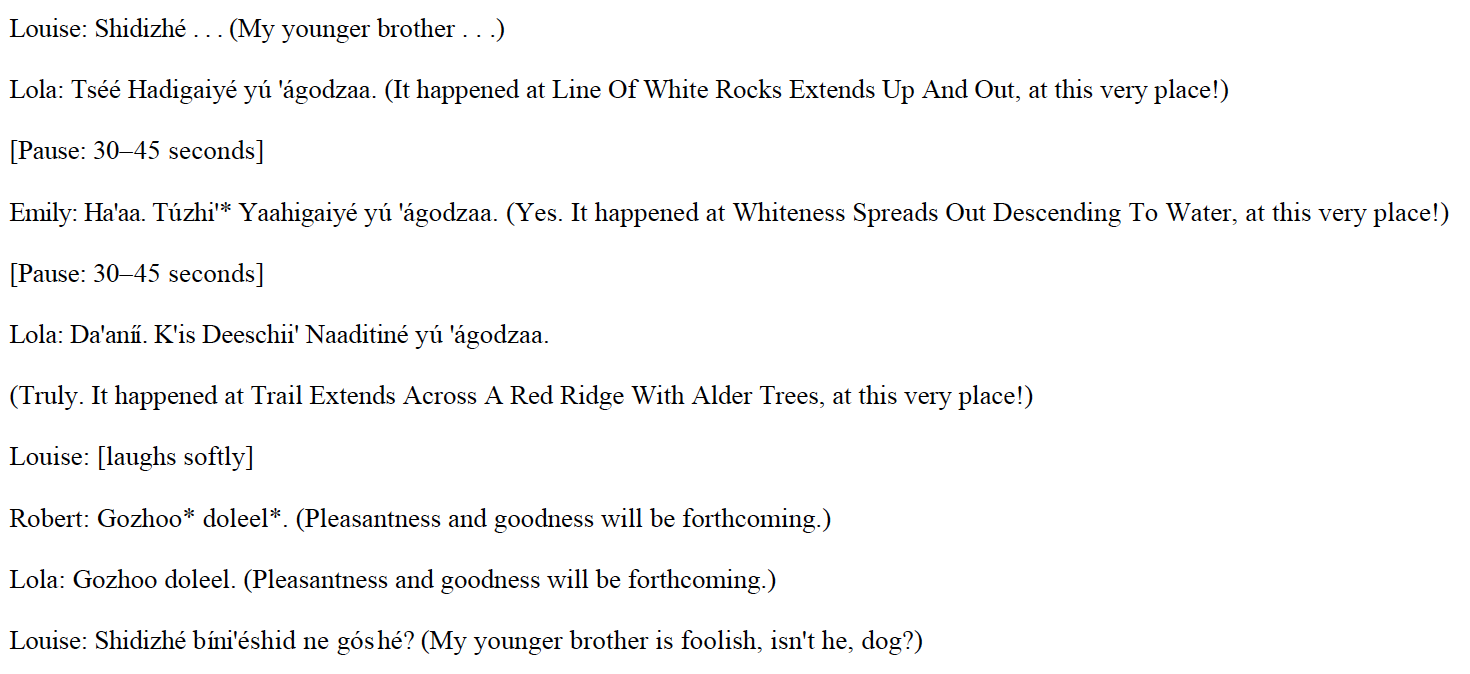
\includegraphics[width=7in]{speaking_names.png}
\end{figure}

As the speakers of this interaction further recalled, this particular conversation was used to uplift the mood of one of the speakers, Louise, whose brother suddenly got sick. Evoking the powerful place-names in a conversation, required Louise to add on to the utterances to create a meaning of this interaction. Basso described this conversation as though these women were giving Louise pictures for her mind to build pleasant thoughts so that she would cheer up about her brother. By leaving out some important details from these expressions, these interlocutors, figuratively speaking, left the canvas somewhat blank so that Louise could fill it in with her own thoughts and depictions, fulfilling the voluntary cooperation principle of the Western Apache conversations. 

Another ethnographic study of Apache in San Carlos contributed two additional non-narrative conversational genres, \textit{yati n\l ke'} or `throwing words around' and re-interpretation of songs \parencite{samuels2004}. Considering that the author of this study was especially concerned with songs and music of Apache, both of these conversational genres were observed at a musical performance, yet both of them can occur in any intimate context where interlocutors are familiar and comfortable with each other. 

\textit{Yati n\l ke'} is a conversational practice in which ``each speaker sequentially grabs hold of something in a previous speaker's utterance and builds a new layer on it by spinning it in a new direction'' \textcite[p. 190]{samuels2004}. Samuels observed such interaction during a local band's ``pompous'' performance of Jimi Hendrix's ``Hey Joe.'' The band excited the small audience with its performance, and someone in the crowd yelled out ``in a cowboy falsetto yodel'' \textit{Raaa-haaa!} (instead of most common ``yee-haa'' or ``yaa-haa''). A band's member picked it up and yelled back ``\textit{Rawhide!}'' referring to the song with this name in which ``yaa-haa'' is a recurring phrase and a TV show with same name. Immediately after this, he changed his response, yelling out \textit{hah\'a\'ai'!}, ``the Western Apache exclamation of delight at another's comeuppance'' (p. 189). This short exchange (12 seconds) consists of multiple expressions connected to each other in participants' imagination: ``the performance of a Jimi Hendrix version of ``Hey Joe,'' a rodeo shout, a popular television show theme song, and a Western Apache interjection'' (p. 190) do not naturally come together for the English speakers, but are easily imaginable in this conversational practice. 

Song re-interpretation is also a performative conversational genre, which seems to occur in intimate settings of small audience or band rehearsal. An example that Samuels provided is that of the rehearsal of Pink Floyd's ``Money,'' which suddenly after the non-verbal introductory riff was sung by everyone in the audience in Apache instead of English. Both English ``money'' and Apache \textit{zhaali} are phonetically similar consisting of two syllables and finishing off on high-front vowel /i/. The group's performance of this song in Apache was only possible in the group itself, Samuels argued: none of the individuals would be able to sing it alone, none knew the lyrics in Apache to the \textit{whole} song. In a sense, song re-interpretation and \textit{yati n\l ke'} are similar conversational genres that share a joking frame and the understanding of the meaning `between speakers' rather than `within an individual.' Structurally they both remind of conversational adjacency pairs, with the first part of the utterance defining the structure of the second one. Functionally, both these genres are not only used for the entertainment of the audience, but for establishing and maintaining solidarity in the small group of speakers. However, what is different between these genres is turn-taking: in ``throwing words around'' speakers are allowed to self-select their turns, while in song re-interpretation, the whole group tends to sing in unison, even without knowing the proper words. 

Examples of these three conversational genres in two Native American communities humbly open the concept of conversational genre continuum for consideration. Once again, in categorization of these speech examples structure and function of talk become the corner stones of distinction. While it would not be too hard to find similar contexts for talk in other speech communities, these examples demonstrate how unique their expressions are. In fact, it takes more than language proficiency to fully understand these exchanges, which indicates that genres are not shared cross-culturally. However, the similarity of the two genres also raises an important point: are genre categorical in the sense of being bound and complete entities, or are they more fluid? In the following section, I suggest that instead of providing a full and complete list of speech genres for a given speech community, it is much more efficient and productive to conceptualize genres as a continuum with fluid borders.

\begin{figure}[ht]
\caption{Continuum of conversational genres.}
\label{continuum}
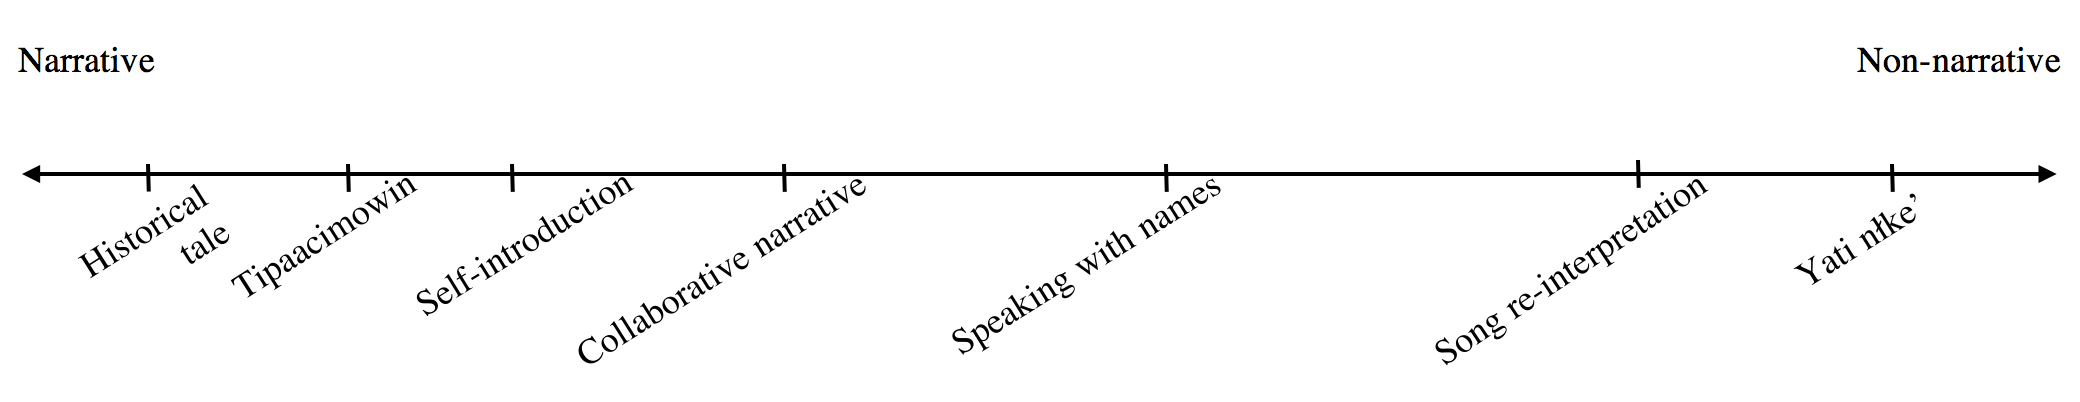
\includegraphics[width=7in]{continuum.png}
\end{figure}

In this section, I wanted to provide some examples of the speech genres of narratives found in different speech communities across North America. Needless to say, this is only a short list that demonstrates the value of genre categorization and the basis for such a distinction. There is no doubt that other conversational genres exist in these and other communities, differing in their structure or functions. From the analytical point of view, such a distinction of conversational genre helps in the analysis of a performance in establishing the ground rules for particular types of storytelling and face-to-face interaction. Rejection of genre rules can be indicative of the necessity to address different social needs or create a new function of a narrative. In other words, genre categorization is especially useful for the understanding of the social functions of an interaction and its meaning in the socio-historical discourse. Another important observation rising from these examples is regarding the cross-cultural variation. Although I included examples from geographically neighboring communities, it is obvious that some structural and functional variations between these genres exist. If one was to compare these genres to what is more familiar to us in the Euro-American culture of the English-speaking world, we would not be able to distinguish exactly the same genres. In fact, I would argue that some of these genres are so unique that they exist only in these speech communities. For example, there is no equivalent of pageant storytelling in English-speaking cultures due to the fact that English is not undergoing language shift and there is no fear of losing the traditional English storytelling. On the contrary, however, a performative conversational narrative in English that is learned and reproduced from memory may exist in a non-English speaking community to increase the linguistic capital of a contestant and demonstrate a transnational identity \parencite{billings2009}. 
\subsection{Person Reference as an index of Conversational Genre}
In their studies of the communicative practices among Western Apache and Severn Ojibwe, \textcite{basso1996,basso1990,valentine1995,samuels2004} noticed particular structural and lexical features accompanying each of the described speech events. Besides the situational time-related adverbs, types of place-names play an important role in the Western Apache conversations, and depending on the type of the evoked place names, speakers are able to navigate the conversational matrix to ensure the particular effect of a conversation. Person reference terms may also act in a similar way due to their adherence to particular structural and cultural principles. So having argued that some types of person reference terms in certain cultures tend to correlate with a particular speech action, one would also expect such terms to be especially recognizable in conversational genres as well. In fact, because of their strong social and conversational (structural) features, person reference forms can better serve as anchors of conversational genres.

An example of how person reference may serve as genre detection tool comes from a research on Northern Pomo conversations and third person reference \parencite{oconnor1990}. In her study, O'Connor examined the types of person references in a short conversational narrative that served a purpose of criticism or complaint. The conversational practice of complaining in Northern Pomo is characterized by a specific grammatical structure involving the verb `to cry' and an oblique argument. Furthermore, this speech type has different genres depending on the responses it elicits from the interlocutors. So, for example, one may complain about about a certain situation or to a higher authority. In the case of the latter, the complaint can be structured in such a way that the hearer may be able to easily discern main parts for a further action to remedy the complaint \parencite[p. 381]{oconnor1990}. What is even more fascinating for the current study, is that O'Connor discovered correlations between the conversational genres of complaint and the person reference terms they use. 

According to \textcite{oconnor1990} there are three major person reference patterns seen in the Northern Pomo complaints. The first important finding pertains to the avoidance of personal names when complaining or criticizing other people. As it has been shown earlier, names are considered both economic and recognitional in conversations, so their use should also associate with instantaneous affect. In Northern Pomo speech community where nearly every one knows one another, using a recognitional person reference form can have a negative effect either on the person, the speaker (for gossiping is not necessarily valued), or their mutual relationships. This complex cultural predispositions to the negative effects of complaint cause speakers to avoid personal names in this conversational genre. Furthermore, avoidance of a name in person reference can serve as an indicator of conversational coherence: only if the hearer fully understands the reasons for name avoidance, they would not question this cultural norm by repair. In other words, an establishment of an identity without a recognitional term in a complaint is a dynamic emergent practice reflecting the social organization.

Use of demonstrative pronoun \textit{mul} in Northern Pomo becomes the most common in complaints. As \textcite{oconnor1990} noted, the demonstrative when used as an enclitic or prenominally does not have inherent negative connotations. Yet, when used independently to refer to adult human beings, it acquires a meaning of derogation, which helps to establish the framework of criticism or complaint. She furthermore argued that the freestanding demonstrative pronouns tend to be important markers of discourse organization, that is they ``cluster in orientation and (to a lesser extent) action sections'' (p. 394). Thus, the structure of a conversation is organized by the person reference form, which can highlight the focus of the complaint and draw attention from the less important participants by assigning them more neutral reference terms. 

The example of Northern Pomo conversation and the analysis of its referential terms indicate an intricate connection between the social structure and the discourse. Choosing certain reference forms, speakers negotiate their social positioning and the social organization of their community of practice. In addition, these reference forms also establish the framework of a conversational genre of complaint in which one party criticizes someone else, and the expectation of the hearer is not to interject with a repair. It is in the context of complaint that some reference terms receive their semantic cues. 
\section{Conclusion}
The discovery of different discourse genres in the Severn Ojibwe speech community, \textcite{valentine1995} encountered some analytical problems. Her main concern was with the concept of genre, and her dissatisfaction with it were in part due to the high variations in her data as well as the multiple approaches available to its analysis. Recognizing that not all of the speech in her data are conversations or narratives, Valentine used different frameworks of analysis and have found it impossible to use either just CA, just ethnopoetics, or just discourse analysis to get to the bottom of the linguistic variation in the discourse. Indeed, it is merely impossible to apply CA to analyze narrative, and one cannot rely on ethnopoetics in the analysis of interaction. However, more than twenty years later, genre studies seem more approachable today at least with the availability of sociocultural linguistics \parencite{bucholtz2008}.

Similarly, because the concept of a conversational genre does not really belong to a single discipline, it allows to bridge the gap between the cultural contexts of a conversation and its interactional features (studied by CA). Person reference is the conversational feature that is grounded both in the organization of the conversation and the cultural premises of talk. Meanwhile, conversational genre as it is defined here form a continuum of possible conversational categories distinguishable by their discourse mode, their structure, and their social function. As ideational concept, it is possible to investigate the conversational genre from the point of view of their effect in the discourse as well as their acceptance (or rejection) in a conversation. As a concept tightly intertwined with the socio-historical functions of discourse, conversational genre can shed the light on the social organization on the ``macro'' level \parencite{mayes2005}. As a link of cultural and structural contexts, person reference in this paper has been presented to be the feature of conversational genre that can serve as a feature defining the conversational genre.
\printbibliography

\end{document}
